\documentclass{standalone}
\usepackage{bera,graphicx,xcolor}

\definecolor{uibkgray}{cmyk}{0,0,0,0.9}

\setlength{\paperwidth}{1440pt}
\setlength{\paperheight}{225pt}
\setlength{\oddsidemargin}{0pt}
\setlength{\topmargin}{0pt}

\begin{document}
\nopagecolor
\sf
\begin{picture}(1440,225)
\put(0,15){\makebox(0,0)[lb]{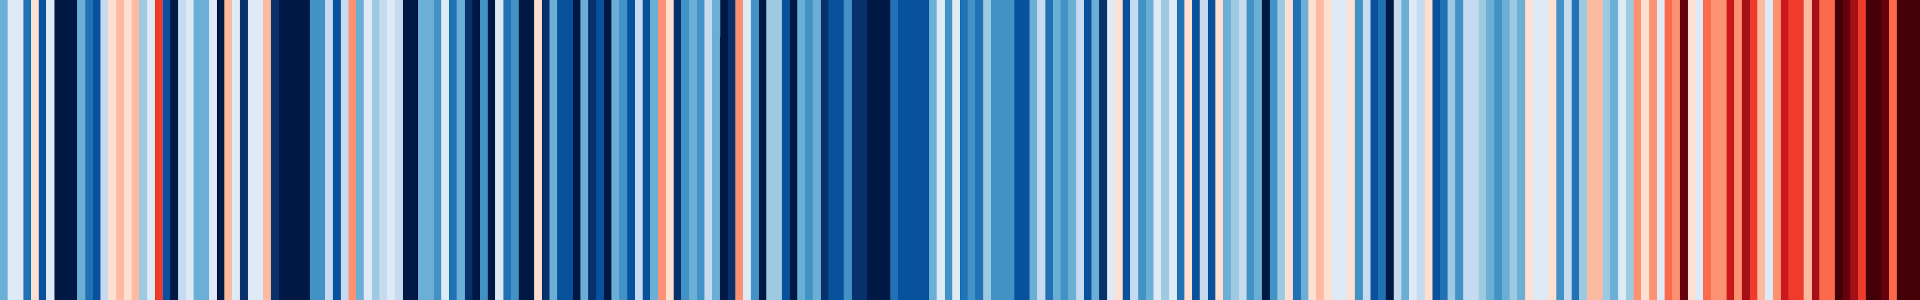
\includegraphics[width=1440pt,height=210pt]{uibk-stripes.png}}}
\put(1420,3){\makebox(0,0)[rb]{\fontsize{10pt}{12pt}\selectfont \textcolor{uibkgray}{\textbf{Source:} ShowYourStripes.info}}}
\end{picture}
\end{document}
